\documentclass[11pt]{article}
\usepackage[margin=2.3cm]{geometry}
\usepackage{amsmath}
\usepackage{tikz}
\usetikzlibrary{arrows.meta,positioning,fit,calc}
\usepackage{listings}
\usepackage{xcolor}
\usepackage{booktabs}
\usepackage{parskip}
\usepackage{hyperref}
\usepackage{titlesec}
\usepackage{enumitem}
\usepackage{fancyhdr}
\usepackage{tcolorbox}
\tcbuselibrary{skins,breakable}

\hypersetup{colorlinks=true,linkcolor=blue!50!black,urlcolor=blue!50!black,citecolor=blue!50!black}
\definecolor{codebg}{RGB}{245,245,245}
\definecolor{accent}{RGB}{20,80,150}

\lstset{
  basicstyle=\ttfamily\small,
  backgroundcolor=\color{codebg},
  breaklines=true,
  frame=single,
  framerule=0.3pt,
  rulecolor=\color{gray!40},
  columns=fullflexible,
  showstringspaces=false,
  xleftmargin=2pt, xrightmargin=2pt,
}

\titleformat{\section}{\large\bfseries\color{accent}}{\thesection}{0.6em}{}
\titleformat{\subsection}{\normalsize\bfseries}{\thesubsection}{0.6em}{}

\pagestyle{fancy}
\fancyhf{}
\fancyhead[L]{\small agent-runtime --- Brief}
\fancyhead[R]{\small\thepage}
\renewcommand{\headrulewidth}{0.3pt}

\newcommand{\code}[1]{\texttt{\small #1}}
\sloppy
\emergencystretch=2.5em

\title{\vspace{-1.5cm}\textbf{\Huge agent-runtime}\\[0.3cm]\Large Brief: an event-sourced runtime for tool-using LLM agents}
\author{Concise, accurate overview for the project owner}
\date{}

\begin{document}
\maketitle
\thispagestyle{empty}

\begin{tcolorbox}[colback=yellow!10,colframe=yellow!50!black,title=Scope of this document,fonttitle=\bfseries]
A condensed, accurate summary of the \code{agent-runtime} project, based only on
its actual code, tests and README. For full detail --- every module, every event
field, every diagram --- see the companion \code{deep-dive.pdf} in the same folder.
\end{tcolorbox}

\tableofcontents
\newpage

\section{What it is, in one paragraph}

\textbf{agent-runtime} is a Python library and CLI (\code{agentrun}) for running
LLM-driven agents (programs that loop: ask a model what to do, run the tool it
requests, feed back the result, repeat) with the operational layer such demos
usually skip: every run is recorded as an append-only \textbf{event log} in SQLite;
the full state of a run is always \emph{computed} from that log, never stored
separately. That one decision buys, uniformly: byte-identical \textbf{replay} of a
past run with no network or tools touched, safe \textbf{resume} after a crash with
no duplicated side effects, a human \textbf{approval gate} before anything with a
side effect executes, deliberate \textbf{failure injection} to prove the loop
degrades cleanly, and a 24-scenario \textbf{regression suite} that pinpoints the
first event where two model/behavior versions diverge.

\section{Architecture}

\begin{center}
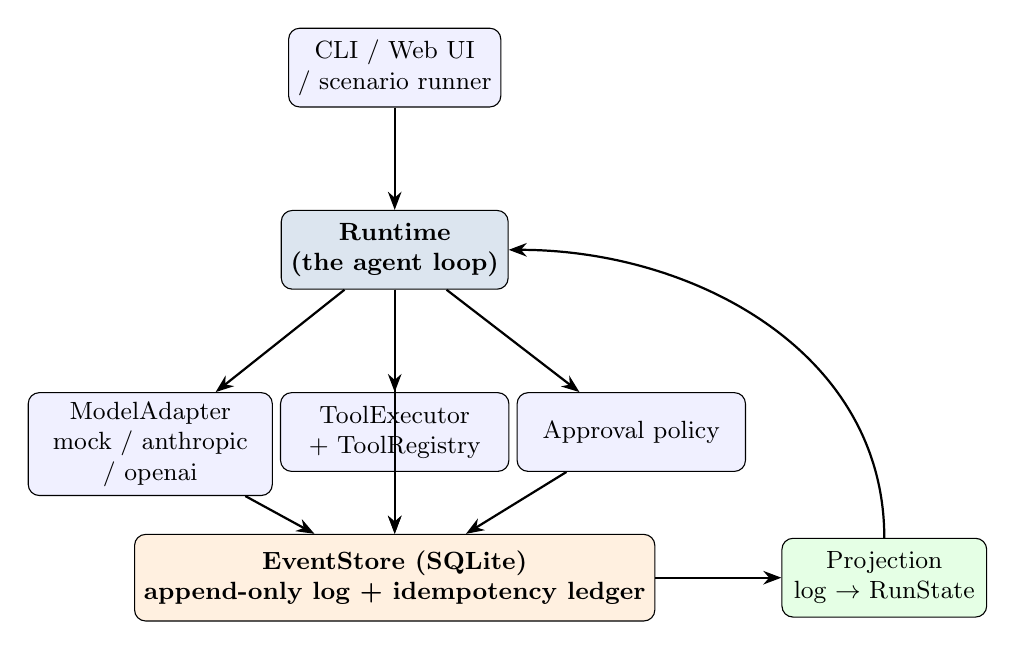
\begin{tikzpicture}[
  box/.style={draw, rounded corners, fill=blue!6, minimum height=1cm, minimum width=2.6cm, align=center, font=\small},
  core/.style={box, fill=accent!15, font=\small\bfseries},
  store/.style={draw, fill=orange!12, minimum height=1.1cm, minimum width=3.6cm, align=center, font=\small\bfseries, rounded corners},
  arr/.style={-{Stealth[length=2.3mm]}, thick},
  node distance=1.0cm and 1.0cm
]
  \node[box] (cli) {CLI / Web UI\\ / scenario runner};
  \node[core, below=1.3cm of cli] (rt) {Runtime\\ (the agent loop)};
  \node[box, below left=1.3cm and 0.1cm of rt, minimum width=3.1cm] (adapter) {ModelAdapter\\ mock / anthropic\\ / openai};
  \node[box, below=1.3cm of rt, minimum width=2.9cm] (exec) {ToolExecutor\\ + ToolRegistry};
  \node[box, below right=1.3cm and 0.1cm of rt, minimum width=2.9cm] (appr) {Approval policy};
  \node[store, below=3.1cm of rt] (store) {EventStore (SQLite)\\ append-only log + idempotency ledger};
  \node[box, right=1.6cm of store, fill=green!10] (proj) {Projection\\ log $\rightarrow$ RunState};

  \draw[arr] (cli) -- (rt);
  \draw[arr] (rt) -- (adapter); \draw[arr] (rt) -- (exec); \draw[arr] (rt) -- (appr);
  \draw[arr] (adapter) -- (store); \draw[arr] (exec) -- (store); \draw[arr] (appr) -- (store);
  \draw[arr] (rt) -- (store);
  \draw[arr] (store) -- (proj);
  \draw[arr] (proj.north) to[out=90,in=0] (rt.east);
\end{tikzpicture}
\end{center}

No SQL statement in \code{store.py} updates or deletes an event row --- only
inserts and selects. \code{projection.py} is the single module that turns a log
into meaning (\code{RunState}); the CLI, web UI, replay comparator and scenario
assertions all consume it, so they can never disagree about a run's status.

\section{The event log}

Table \code{events(run\_id, seq, type, ts, payload)}, primary key
\code{(run\_id, seq)}. Twelve event types cover a run's whole life:
\code{run\_created}, \code{model\_requested}, \code{model\_responded},
\code{model\_error}, \code{tool\_requested}, \code{tool\_approved}/\code{tool\_denied},
\code{tool\_executed}/\code{tool\_failed}, \code{checkpoint},
\code{run\_finished}/\code{run\_failed}. Every event has a \emph{canonical} JSON
encoding (sorted keys, no whitespace) so two logs can be compared for exact
equality --- this is what lets replay claim ``byte-identical.''

\section{The loop}

\code{Runtime.drive(run\_id)} repeats: project the log $\to$ if terminal, stop;
resolve pending tool calls in order (read-only ones execute; side-effecting ones
need an approval decision, or the loop pauses as \code{waiting\_approval}); if
nothing pending and under the call limit, ask the model for the next turn, append
what happened, loop. Because every step is recomputed from the log, ``resume after
a crash'' and ``continue after a human approves'' are the \emph{same} code path as
an ordinary iteration --- there is no separate recovery logic.

Conversation reconstruction (\code{build\_messages()}) is likewise a pure function
of the log: system prompt, request, then one message per subsequent model turn or
tool observation. A denial becomes a \code{\{"denied": true, "reason": ...\}}
observation the model can react to; malformed output becomes a corrective
``please reply with tool calls or a final answer'' message.

\section{Idempotency and crash safety}

Side effects must not repeat on resume. The executor derives a key from
\code{(run\_id, seq of the tool\_requested event)} --- stable across a crash and
resume --- and writes the result to an \code{INSERT OR IGNORE} ledger
\emph{before} the runtime appends \code{tool\_executed}. If the process dies in
between (the crash window), a resumed run finds the ledger entry and reports
\code{replayed: true} instead of re-running the handler. \code{tests/test\_resume.py}
crashes a run at exactly that instant and asserts a side-effect counter stays at 1.

\section{Deterministic replay}

\code{agentrun replay <run-id>} rebuilds a run using four \emph{recorded} stand-ins
--- a clock, an adapter, a tool executor and an approval policy --- each replaying
only what the original log recorded, with no network, tool handler or key needed.
The real, unmodified runtime then drives the loop, and the two canonical logs are
compared; any difference is reported as the exact first diverging event sequence
number. \code{--until <seq>} truncates the source log for stepwise debugging.

\section{Failure injection}

A YAML-declarable \code{FaultPlan} names faults at specific points: model faults
per adapter call (\code{malformed}, \code{adapter\_500}) and tool faults per
attempt (\code{timeout}, \code{exception}). The runtime's contract: adapter errors
retry with exponential backoff then fail the run with a cause; malformed output
gets two corrective retries then fails; tool failures surface to the model as
ordinary error observations. Nothing escapes \code{drive()} as an unhandled
exception --- \code{tests/test\_faults.py} pins this down.

\section{Cost accounting}

Every \code{model\_responded} event carries token usage and latency.
\code{accounting.py} folds these into a per-run cost using a small, hardcoded
price table (the project's own README flags this table as something that ``will
drift''). The mock adapter's usage numbers are fabricated deterministically from
message size and always marked \code{simulated: true} in the CLI and web UI.

\section{Tools}

Each tool declares a JSON-schema for its arguments, a \code{side\_effect} flag, a
timeout and a retry budget (\code{tools/registry.py}). The executor validates
arguments, runs the handler with a timeout, and retries transient failures with
backoff while failing fast on expected, deterministic ones (\code{ToolError}). All
file paths are sandboxed to the run's workspace directory.

\begin{center}
\small
\begin{tabular}{@{}p{2.6cm}p{7.3cm}p{1.6cm}@{}}
\toprule
\textbf{Tool} & \textbf{What it does} & \textbf{Side effect} \\
\midrule
\code{read\_file} & read a UTF-8 text file & no \\
\code{write\_file} & write a UTF-8 text file & yes \\
\code{list\_files} & recursively list files & no \\
\code{http\_get} & GET an allowlisted URL & no \\
\code{csv\_update} & append a row / set a cell in a CSV & yes \\
\code{draft\_email} & write a \code{.eml} draft file --- never sends & yes \\
\code{calendar\_add} & insert a row into a per-workspace SQLite calendar & yes \\
\code{calendar\_list} & read the calendar back & no \\
\bottomrule
\end{tabular}
\end{center}

\section{Model adapters}

One interface, \code{ModelAdapter.complete(messages, tools) -> ModelTurn}, three
implementations: \code{MockModelAdapter} (a deterministic, offline script player
used by tests and scenarios --- see Sec.\,10), \code{AnthropicAdapter} (Messages
API) and \code{OpenAIAdapter} (Chat Completions API), both env-key-driven via
\code{httpx}.

\begin{tcolorbox}[colback=red!6,colframe=red!50!black,title={Honest scope note (verbatim from the README)},fonttitle=\bfseries\small]
``The Anthropic and OpenAI adapters are implemented against their current APIs and
covered by offline contract tests (request building, response parsing, error
mapping via injected HTTP transports), but no live API calls were made here
because no API keys were available. Everything else, including the full test
suite, the CLI and the web UI, runs and was verified entirely offline.''
\end{tcolorbox}

\section{Agents and scenarios}

Three example agents, each a fixed system prompt and a restricted tool subset:
\code{ops\_assistant} (chases overdue invoices, drafts reminder emails, never
sends), \code{data\_entry} (transcribes records into CSV, verifies by reading
back), \code{research\_summarizer} (fetches allowlisted pages/notes, writes a
sourced summary). 24 YAML scenario files ship under \code{scenarios/}, 8 per
agent, each scripting one or more named \emph{behavior} versions for the mock
adapter plus an \code{expect} block of assertions (exact/contains tool lists,
denied tools, final-answer substrings, failure cause, files created, minimum
event count, and a structural check that no side effect ever executed before its
approval). \code{agentrun test scenarios/ --behavior v1 --compare v2} runs both
versions and reports the first event where their behavior diverges --- a
regression tripwire for model or prompt changes.

\section{CLI and web UI}

\code{agentrun run/resume/replay/runs/approvals/test/serve/agents} cover starting
and inspecting runs, replay, the approval queue, the regression suite, and a small
FastAPI web UI (\code{agentrun serve}) that lists runs, shows a run's timeline, and
renders pending approvals as human-readable \textbf{diff-style previews}
(\code{web/preview.py}, a real unified diff for file/CSV writes, a plain
\code{+}-prefixed summary for actions with no natural ``before'' state) before a
human clicks approve or deny.

\begin{tcolorbox}[colback=red!6,colframe=red!50!black,title={Known limitation (from the README)},fonttitle=\bfseries\small]
``Approvals via the web UI resume the run synchronously inside the request
handler. A slow tool blocks the HTTP worker for its whole timeout. A real
deployment needs a worker process consuming a resume queue, with the UI only
appending decision events.''
\end{tcolorbox}

\section{Testing}

93 test functions across 13 files, all offline --- confirmed directly from the
files present in \code{tests/}, matching the README's own count (``93 tests, all
offline''). No test makes a live call to Anthropic or OpenAI.

\section{Honest limitations, in the project's own words}

\begin{itemize}[nosep]
  \item Tool timeouts abandon a worker thread rather than kill it (a
  \code{concurrent.futures} limitation); a genuinely hung tool leaks a thread per
  attempt.
  \item Resume repositions the mock adapter's script/fault counters by counting
  events; correct for the tested states, but could realign an injected fault
  sequence off by one in an untested edge case.
  \item Event payloads carry no schema version --- replay is a divergence
  tripwire today, not a migration story.
  \item The cost table in \code{accounting.py} is hardcoded and will drift; the
  in-house neutral message format ignores streaming and provider-specific
  parallel tool-call semantics.
\end{itemize}

\section{Glossary}
\begin{description}[leftmargin=3.2cm, style=nextline]
\item[Event sourcing] Storing every state change as an immutable ordered log, and
computing current state from it on demand, instead of overwriting stored state.
\item[Idempotent] Doing something twice has the same effect as doing it once.
\item[Replay] Re-driving logic using only recorded data, no live calls, checking
the result matches what was recorded.
\item[Side effect] An action with a lasting, observable consequence outside the
program (writing a file, sending an email).
\item[Sandbox] A restricted environment limiting what a program can access.
\item[Contract test] A test verifying request/response shape against a real API's
spec without calling the real API.
\end{description}

\end{document}
